% Chapter 2
\chapter{Piste n° 1} % Main chapter title
\label{Chapter2} % For referencing the chapter elsewhere, use \ref{Chapter2}
%----------------------------------------------------------------------------------------

\begin{description}
  \item[Version du Kernel :] 3.14
  \item[Code de travail :] imx219.c (fichier de la solution 2 sur le rapport du
  09/01/2017)
\end{description}

Suite à l'exploration de 3 pistes, nous avons choisi de nous
concentrer sur la solution n°2 dont le driver compile sans erreur mais ne
réussit pas le chargement.

\section{Erreur}
Constat : Le driver apparait à la commande lsmod mais est inutilisé.

\begin{figure}[th]
   \centering
   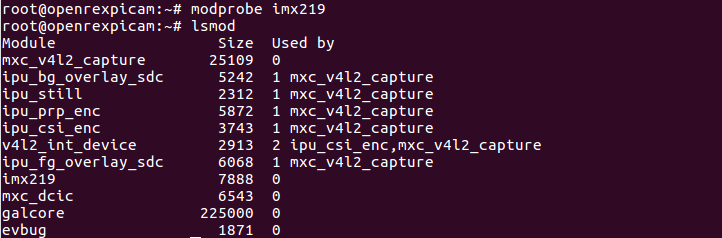
\includegraphics[width=1\linewidth]{chargement_driver.png}
   \decoRule
   \caption{Chargement du module}  \label{fig:planning}
\end{figure}

Après recherche d'indices pour le debug, on retient le message d'erreur suivant:
\begin{figure}[th]
  \centering
  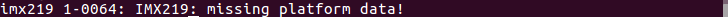
\includegraphics[width=1\linewidth]{errorplatform_dta.png}
  \decoRule
  \caption{Debug probe}  \label{fig:planning}
\end{figure}

Résultat de l'annalyse :
l'erreur provient des premières lignes de la première fonction probe du driver. La
sécurité testant le premier paramètre d'appel du driver s'est déclanchée. le
paramètre est une structure contenant des informations sur les périphériques i2c.
Il y a donc problème de compatibilité entre le driver imx219 et le gestionnaire i2c. Selon
l'avis de notre professeur de yocto qui a été appuyé par nos recherches,
le driver en question utilise les interfaces de fonctionnement nommées
platform\_data, technologie remplacée progressivement depuis 2011 par le
device-tree et sa gestion des compatibilités.

\section{Solution}
Aujourd'hui mardi 16 janvier nous avons cherché à porter le driver vers
une compatibilité avec le device-tree.
\begin{description}

  \item[Ajout de la structure type of\_device\_id dans le driver]

  \begin{lstlisting}
  static const struct of_device_id imx219_of_match[] = {
    { .compatible = "sony,imx219", .data = 0 },
    {}
  };

  MODULE_DEVICE_TABLE(of, imx219_of_match);
  \end{lstlisting}

  \item[Completion de la structure de manipulation du driver]

  \begin{lstlisting}
  static struct i2c_driver imx219_i2c_driver = {
    .driver = {
      .name = "imx219",
      .of_match_table = of_match_ptr(imx219_of_match),
    },
    .probe		= imx219_probe,
    .remove	= imx219_remove,
    .id_table	= imx219_id,
  };
  \end{lstlisting}

  \item[Suppression de la sécuritée platform data]
  \begin{lstlisting}
    if (!ssdd) {
      dev_err(&client->dev, "IMX219: missing platform data!\n");
      return -EINVAL;
    }
    \end{lstlisting}
\end{description}

\section{Conclusion}
Une nouvelle erreur est apparue cependant les travaux qui concernant le
device tree ont fonctionné correctement car on peut remarquer au démarage
que le driver est chargé automatiquement.

\section{Erreur}
Au chargement de la nouvelle image nous obtenons les erreur suivantes:

\begin{figure}[th]
  \centering
  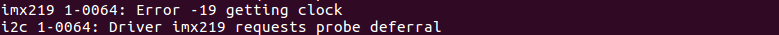
\includegraphics[width=1\linewidth]{errorclk.png}
  \decoRule
  \caption{Debug probe}  \label{fig:planning}
\end{figure}

L'erreur est relative à la fonction getclk du driver qui est une sécuritée tout comme la fonction suprimer précedement.
Elle confimre que nous avons des dificultés à communiquer avec l'i2c.

\section{Solution}
Notre strategie est de supprimer cette nouvelle fonction de securitée, pour avoir plus
d'informations sur la façon dont le driver fonctionne.
\begin{description}
  \item[Suppression de la securitée d'horloge]
    \begin{lstlisting}
	  if (IS_ERR(priv->clk)) {
		    dev_info(&client->dev, "Error %ld getting clock\n",
			  PTR_ERR(priv->clk));
		    return -EPROBE_DEFER;
	  }
    \end{lstlisting}
\section{Conclusion}
Le driver est maintenant charger "correctement" par le kernel.

\begin{figure}[th]
  \centering
  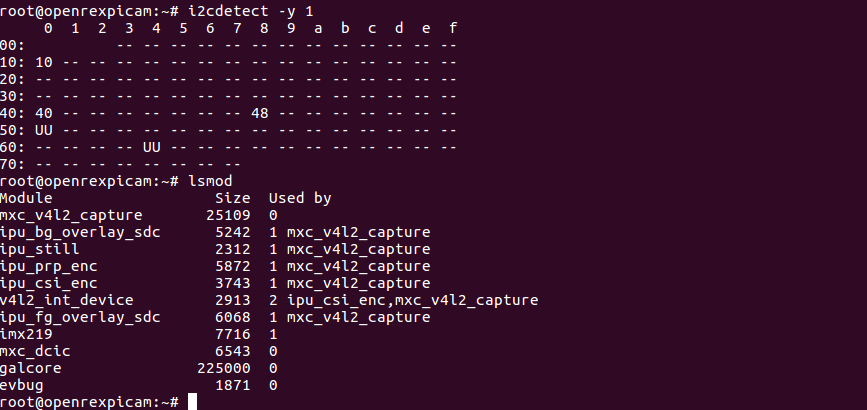
\includegraphics[width=1\linewidth]{lsmodeti2cdetect.png}
  \decoRule
  \caption{Debug probe}  \label{fig:planning}
\end{figure}

    \clearpage
  \end{description}

    \section{Conclusion}
  On peut voir que l'i2c peut maintenant utiliser le dirver imx219 et
  qu'il est utilisé par un autre module. Nous ne sommes toujours pas en mesure
  d'utiliser le driver car les informations sur son utilisation nous manque.
  Deplus de nouvelles erreurs apparaissent au chargement du driver.

  \section{Erreur}
  Au chargement du driver nous obtenons le debug suivant:

  \begin{figure}[th]
    \centering
    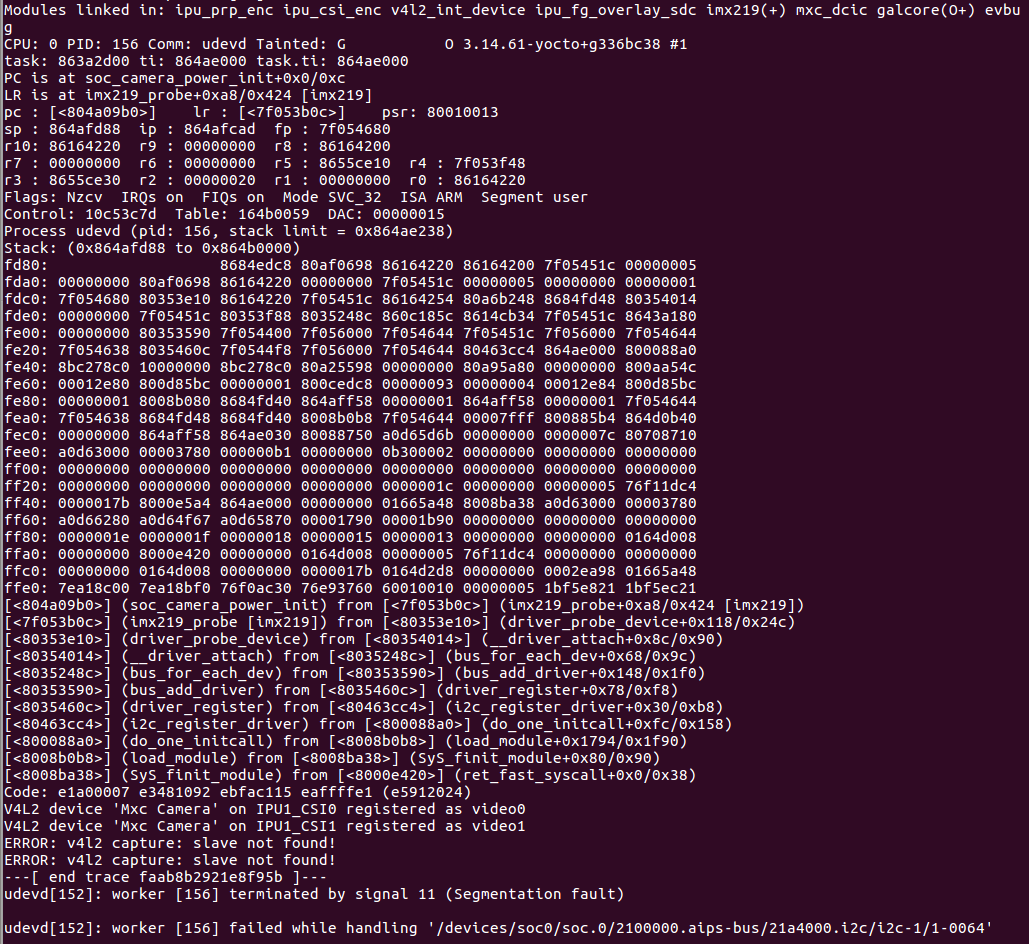
\includegraphics[width=1\linewidth]{debugdmesg.png}
    \decoRule
    \caption{Debug probe}  \label{fig:planning}
  \end{figure}

  \section{Reste à faire}

   Determiner la cause du segmentation fault.

\begin{figure}[th]
  \centering
  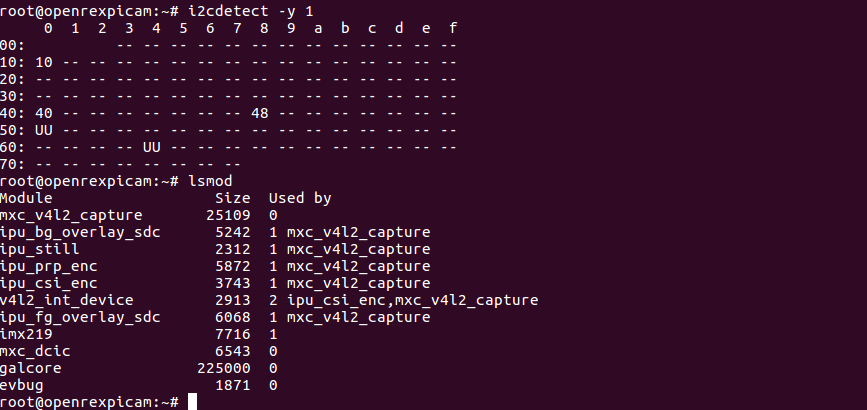
\includegraphics[width=1\linewidth]{lsmodeti2cdetect.png}
  \decoRule
  \caption{Debug probe}  \label{fig:planning}
\end{figure}

    \clearpage
  \end{description}

  On peut voir que l'i2c peut maintenant utiliser le dirver imx219 et
  qu'il est utilisé par un autre module. Nous ne sommes toujours pas en mesure
  d'utiliser le driver car les informations sur son utilisation nous manque.
  Deplus de nouvelles erreurs apparaissent au chargement du driver.

  \section{Erreur}
  Au chargement du driver nous obtenons le debug suivant:

  \begin{figure}[th]
    \centering
    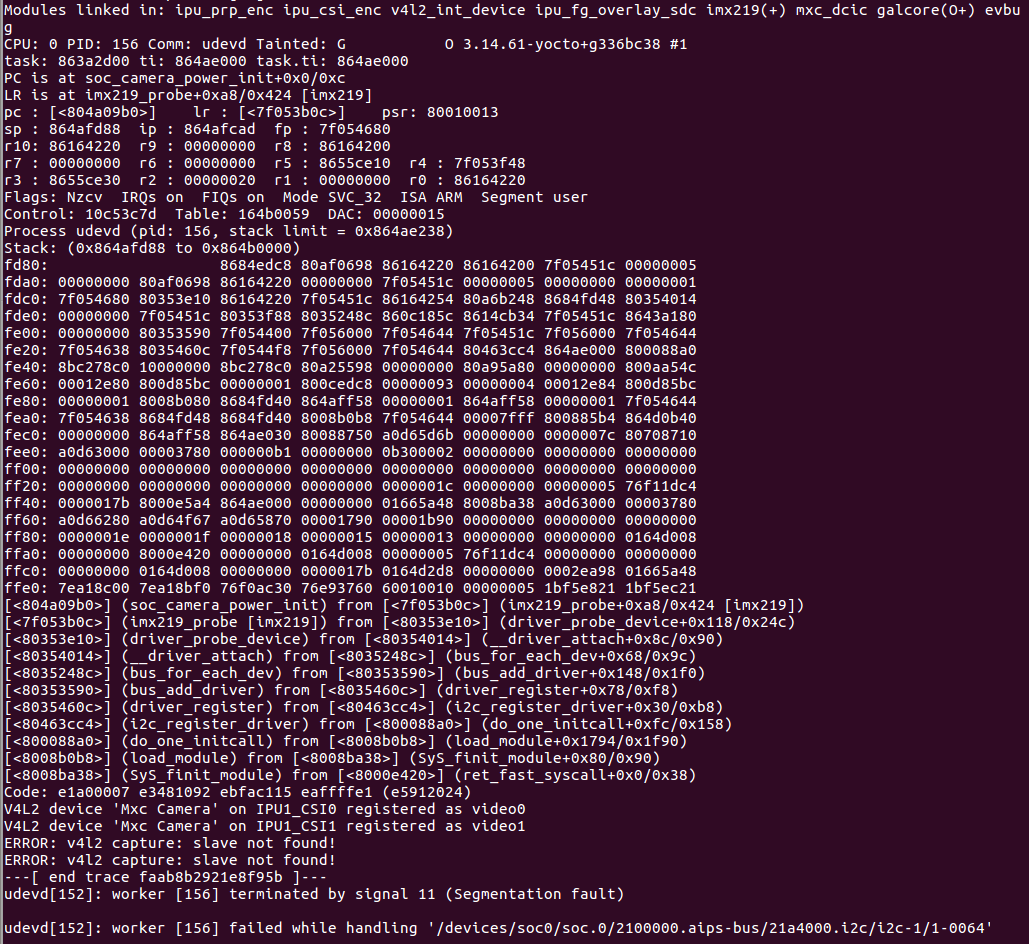
\includegraphics[width=1\linewidth]{debugdmesg.png}
    \decoRule
    \caption{Debug probe}  \label{fig:planning}
  \end{figure}

  \section{Reste à faire}

   Determiner la cause du segmentation fault.

   Savoir comment recuperer le flux video.

    %----------------------------------------------------------------------------------------
